% !TeX encoding=utf8
% !TeX spellcheck = de-CH


\chapter{Applikation}

Dieses Kapitel beschreibt den Entwicklungsverlauf unserer Applikation, die
zugrundeliegenden Algorithmen und Datenstrukturen sowie das Klassenmodell und
die Interaktionen zwischen den verschiedenen Applikationsschichten.

Programmausschnitte werden  in Python-Code wiedergegeben.

\section{Algorithmus}\label{sec:algorithm}

Der ACO-Algorithmus ist in den Grundzügen einfach. Eine gewisse Anzahl autonomer
Agenten (Ameisen) bewegt sich ausgehend von einem Nest-Knoten entlang eines
Graphen bis zu einem Futter-Knoten. Die Ameise muss sich bei jedem Knoten
entscheiden, über welche Kante sie zum nächsten Knoten gelangen möchte. Diese
Entscheidung basiert hauptsächlich auf der Menge an Pheromonen, die sich auf
dieser Kante befindet. Dies wird wiederholt, bis die Ameise den Futterknoten
erreicht. Danach befindet sie sich auf dem Rückweg zum Nest. Sie geht denselben
Weg, den sie gekommen ist, zurück und erhöht jeweils die Pheromonwerte auf den
Kanten, die sie benutzt. Wenn sie das Nest erreicht hat, wird sie erneut auf den
Weg geschickt.

Programmiert könnte der Algorithmus etwa so aussehen:

\lstset{language=Python} 
\begin{lstlisting} 
def ant_algorithm(ants, graph): 
	for ant in ants: 
		next_edge = choose_next_edge(ant.node, graph) 
		ant.node = next_edge.other_node(ant.node) 
		if ant.has_solution:
			ant.update_phermone_trail(next_edge) 
	evaporate_pheromones(graph)
	reset_ants_with_solution(ants) 
\end{lstlisting}

\noindent Wichtig sind die verschiedenen Funktionen, die in diesem
kurzen Codeblock aufgerufen werden:

\begin{description} \item[choose\_next\_edge] Bestimmt auf der Grundlage von
verschiedenen Parametern, die wir jetzt noch nicht kennen, welche Kante die
Ameise als nächstes besuchen wird. \item[update\_pheromone\_trail] Erhöht die
Pheromonmenge auf einer Kante des Graphen. \item[evaporate\_pheromones]
Verringert die Menge an Pheromonen auf einer Kante des Graphen.
\item[reset\_ants\_with\_solution] Die Ameisen, die mit einer fertigen Lösung
wieder beim Nest angekommen sind, werden zurückgesetzt und können
wiederverwendet werden. \end{description}

\subsection{Ablauf und Berechnungen}

Für die verschiedenen Teilschritte sind ein paar wenige, einfache Formeln zu
verwenden. Sie werden benötigt um

\begin{itemize} \item zu ermitteln, welche Wahrscheinlichkeit einzelne Kanten
haben, als nächstes von einer Ameise ausgewählt zu werden, \item die Menge an
Pheromonen zu bestimmen, die eine Ameise auf einer Kante hinterlässt und \item
die Pheromonmenge nach der Evaporation zu berechnen. \end{itemize}

\noindent Für die Betrachtung der verschiedenen Formeln soll der folgende Graph
als Grundlage dienen: \\

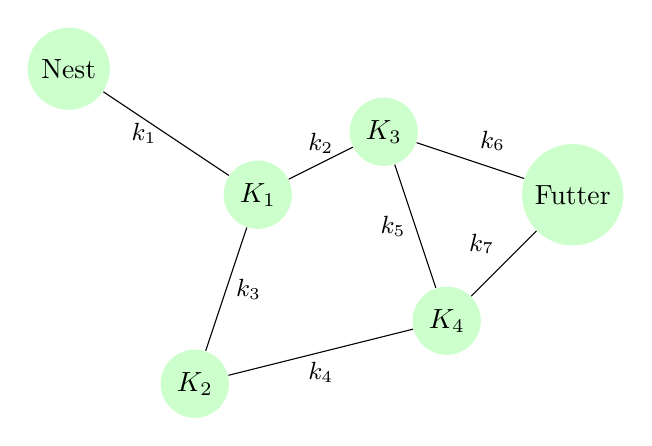
\begin{tikzpicture} [scale=.8,auto=left,every
node/.style={circle,fill=green!20}] \node (nn) at (3,10) {Nest}; \node (n1) at
(6,8)  {$K_1$}; \node (n3) at (8,9)  {$K_3$}; \node (nf) at (11,8) {Futter};
\node (n4) at (9,6)  {$K_4$}; \node (n2) at (5,5)  {$K_2$};

  \path[every node/.style={font=\sffamily\small}] (nn) edge node [left] {$k_1$}
  (n1) (n1) edge node [right] {$k_3$} (n2) edge node [above] {$k_2$} (n3) (n2)
  edge node [below] {$k_4$} (n4) (n3) edge node [left] {$k_5$} (n4) edge node
  [above right] {$k_6$} (nf) (n4) edge node [above left] {$k_7$} (nf);
  \end{tikzpicture}

\subsubsection*{Exploration (Erkundung)}

Solange die Ameise keinen Futterknoten gefunden hat, befindet sie sich in der
Explorationsphase (Erkundungsphase). Wir nehmen an, dass sie sich momentan beim
Knoten $K_1$ befindet. Sie hat bis dahin bereits den Knoten $\{Nest\}$ besucht.
Um Loops zu vermeiden, ist es einer Ameise nicht gestattet, einen Knoten zweimal
zu besuchen. Die Menge der begehbaren Kanten ist demnach $\{k_2, k_3\}$. Die
Pheromonwerte an den beiden Kanten sind $\{phero_{k_2}, phero_{k_3}\}$.

Die Wahrscheinlichkeit für das Begehen einer Kante berechnet sich durch:

\[ p_{k_x} = \frac{phero_{k_x}^\alpha}{\sum\nolimits_{i=0}^n phero_{k_i}^\alpha}
\]

\noindent Der Exponent $\alpha$ ist eine experimentell festgestellte Grösse und
wird in der Literatur mit $2$ angegeben. Um den Exponenten vernünftig anwenden
zu können, müssen sich die Pheromonwerte zwischen $0$ und $1$ befinden,
ansonsten ist das Resultat nicht kontrollierbar. Dies wird erreicht, indem man die
maximale Menge an Pheromonen $phero_{max}$ auf den zur Auswahl stehenden Kanten
ermittelt und folgende Formel auf alle Pheromonwerte anwendet. Als untere Grenze
($phero_{min}$) wird jeweils $0$ verwendet.

\[ phero_{k_i} = \frac{phero_{k_i} - phero_{min}}{phero_{max} - phero_{min}} \]

\noindent Wie man gleich an einem Rechenbeispiel erkennen kann, verstärkt der
Exponent $\alpha$ die Unterschiede zwischen den Pheromonwerten.

\paragraph*{Rechenbeispiel}

Wir betrachten immer noch den obigen Fall und nehmen für die Pheromonwerte der
Kanten $k_2$ und $k_3$ die Werte $phero_{k_2} = 15 $ und $phero_{k_3} = 46$ an.
Zuerst müssen wir diese Werte auf Zahlen zwischen $0$ und $1$ normieren:

\begin{equation*} \begin{split} phero_{k_2} & = \frac{phero_{k_2} -
phero_{min}}{phero_{max} - phero_{min}} \\ & = \frac{15 - 0}{46 - 0} \\ & = 0.37
\end{split} \end{equation*}

\begin{equation*} \begin{split} phero_{k_3} & = \frac{phero_{k_3} -
phero_{min}}{phero_{max} - phero_{min}} \\ & = \frac{46 - 0}{46 - 0} \\ & = 1
\end{split} \end{equation*}

\noindent Ohne $\alpha$ zu beachten, wären die Zähler der
Wahrscheinlichkeitsformel nun $0.37$ und $1$. Die Differenz ist demnach $1 -
0.37 = 0.63$. Wenn $\alpha = 2$ verwendet wird, betragen die Werte $0.37^2 =
0.1369$ und $1^2 = 1$. Die Differenz ist nun $1 - 0.1369 = 0.8631$. Es wird also
wahrscheinlicher, dass $k_3$ te Kante gewählt wird.

Die berechneten Wahrscheinlichkeiten für beide Kanten betragen mit $\alpha = 2$:

\begin{equation*} 
\begin{split} 
p_{k_2} & = \frac{0.37^2}{0.37^2 + 1^2} \\ 
& =0.12 
\end{split} 
\end{equation*}

\begin{equation*} 
\begin{split} 
p_{k_3} & = \frac{1^2}{0.37^2 + 1^2} \\ 
& = 0.88
\end{split} 
\end{equation*}

\noindent Die Kante $k_3$ hat demnach eine ca. siebenmal höhere Chance, als
nächste ausgewählt zu werden.

Um die nächste Kante tatsächlich auswählen zu können, werden die
Wahrscheinlichkeiten gewichtet und durch eine Zufallszahl ausgewählt. Dazu wird
zuerst ein $n$-Tupel der Form $(p_0, p_0 + p_1, p_0 + p_1 + p_2, ...,
\sum\nolimits_{i=0}^n p_n)$ erstellt. Danach generiert man eine Zufallszahl
zwischen $0$ und $1$ und ermittelt mittels Bisektion den korrespondierenden Wert
im Tupel. Unser Tupel besteht nur aus zwei Einträgen $(0.12, 0.12 + 0.88) =
(0.12, 1)$. $k_2$ wird ausgewählt, wenn die Zufallszahl $z \in [0, 0.12)$,
$k_3$, falls $z \in [0.12, 1)$.

\paragraph*{Erweiterung}

Die oben aufgeführte Formel zur Berechnung der Wahrscheinlichkeit lässt sich auf
einfache Weise durch einen bekannten Wert erweitern und beinflussen. In unserem
Fall sind das die Kosten der jeweiligen Kante $cost_{k_i}$. Die Kosten sollen
die Wahrscheinlichkeit gegebenenfalls nach unten korrigieren. Die angepasste
Formel lautet:

\[ p_{k_i} = \frac{phero_{k_i}^\alpha \cdot
cost_{k_i}^\beta}{\sum\nolimits_{i=0}^n phero_{k_i}^\alpha \cdot
cost_{k_i}^\beta} \]

\noindent Auch hier müssen die Kosten normiert werden. Das Ziel ist, die
Wahrscheinlichkeit stärker zu verringern, je grösser die Kosten der
entsprechenden Kante sind. Das heisst, dass, wenn der Kostenwert zwischen $0$
und $1$ normiert wird, höhere Kosten näher bei $0$ und tiefere näher bei $1$
sein müssen. Dies wird durch die folgende Normierungsformel erreicht:

\[ cost_{k_i} = \frac{1}{\frac{cost_{k_i}}{cost_{min}}} \]

\noindent Für dieses Beispiel seien $cost_{k_2} = 10$ und $cost_{k_3} = 20$. In
unserem Beispiel sind die neuen Kosten demnach

\begin{equation*} 
\begin{split} 
cost_{k_2} & = \frac{1}{\frac{10}{10}} \\ 
		   & = 1
\end{split} 
\end{equation*}

\begin{equation*}
\begin{split} 
cost_{k_3} & = \frac{1}{\frac{20}{10}} \\ 
           & = \frac{10}{20} & = 0.5 
\end{split} 
\end{equation*}

\noindent Das bedeutet, dass bei der Auswertung der Wahrscheinlichkeit von $k_3$
die Pheromonwerte mit $0.5$ multipliziert und dadurch verringert werden. Die
Unterschiede zwischen den Kosten-Modifikatoren können durch $\beta$ beeinflusst
werden. Hohe Werte verstärken die Unterschiede, Werte zwischen $0$ und $1$
verringern sie.

\subsubsection*{Exploitation (Verwertung)}

Die zweite Phase des Algorithmus ist die Verwertung des Ergebnisses. Sie
beginnt, wenn die Ameise den Futterknoten erreicht hat. Ab diesem Zeitpunkt geht
sie den von ihr gefundenen Pfad zurück und erhöht die Pheromonmenge auf jeder
Kante, der sie entlangläuft.

Die Menge an Pheromonen ($phero_{inc}$), die zu der bestehenden hinzu addiert
wird, hängt dabei direkt von der gefundenen Pfadlänge ($pathlength$) ab:

\[ phero_{inc} = \left({\frac{1}{pathlength}}\right)^\gamma \]

\noindent Der neue Pheromonwert beträgt danach

\[ phero_{k_i} = phero_{k_i} + phero_{inc} \]

\noindent Das heisst, dass bei längeren Pfaden generell weniger Pheromone
platziert werden. Der Exponent $\gamma$ verstärkt die Unterschiede zwischen den
Mengen, genau wie das $\alpha$ und $\beta$ in der Formel zur Berechnung der
Wahrscheinlichkeiten tun. Die Pfadlänge muss immer $> 1$ sein. Dies kann bei der
Erstellung des Graphen sichergestellt werden.

Sobald die Ameise das Nest erreicht, verliert sie die aktuelle Lösung, und
beginnt wieder von vorn.

\paragraph*{Erweiterung}

Eine sinnvolle, auch von uns implementierte Erweiterung ist die Reduzierung der
addierten Menge an Pheromonen, falls sich bereits eine grosse Menge auf der
Kante befindet. Dies verhindert, dass auf einer Kante immer mehr Pheromone
abgelagert werden, was dazu führen würde, dass andere Kanten keine Chance mehr
hätten, ausgewählt zu werden.

Dazu berechnen wir einen Multiplikator. Der Multiplikator soll nah an $0$ sein,
wenn die sich bereits auf der Kante befindende Menge an Pheromonen gross ist,
und nah an $1$, wenn dieser Wert klein ist.

Ferner wird zu jeder Zeit die Pheromonmenge der Kante mit den meisten Pheromonen
über den gesamten Graph hinweg gesehen in  $phero_{max}$ gespeichert. Die Menge
auf einer spezifischen Kante ist $phero_{k_i}$. Daraus errechnet sich folgender
Multiplikator:

\[ phero_{mul} = \left({ 1 - \frac{phero_{k_i}}{phero_{max}}}\right)^\delta \]

\noindent Dies führt zu folgender Formel zur Berechnung der Menge an Pheromonen,
die zur bestehenden hinzu addiert werden soll:

\[ phero_{inc} = phero_{inc} \cdot phero_{mul} \]

\noindent $\delta$ kann, wie bereits mehrmals erwähnt, zur Gewichtung verwendet
werden und beträgt in unserer Implementation standardmässig $0.1$.

Rechenbeispiel: Die maximale Menge an Pheromonen im Graph sei $phero_{max} =
13$, die Mengen auf den Knoten $k_1 = 5$ und $k_2 = 12$. Das ergibt für
$phero_{mul_{k_1}} = 1 - \frac{5}{13} = 0.62$ und $phero_{mul_{k_2}} = 1 -
\frac{12}{13} = 0.08$. Man sieht, dass auf die Kante mit höherer Konzentration
viel weniger dazu addiert wird als auf die mit der geringeren Konzentration.

\subsubsection*{Evaporation (Verdunstung)}

Im letzten Schritt werden die Pheromonwerte auf allen Kanten verringert. Die
Verringerung ist kein absoluter Wert, ansonsten würden früher oder später Zahlen
$< 0$ erreicht. Daher errechnet sich der neue Pheromonwert einer Kante bei einer
Reduktion von $phero_{red} \in [0, 1]$ durch

\[ phero_{k_i} = (1 - phero_{red}) \cdot phero_{k_i} \]

\noindent Das ergibt z.B. bei einer Pheromonmenge $phero_{k_i} = 10$ und
$phero_{red} = 0.01$ einen neuen Wert von $phero_{k_i} = 0.99 \cdot 10 = 9.9$.
$0.01$ ist zugleich der in der Literatur empfohlene Standardwert für die
Reduktion.

\subsection{Warum funktioniert der Algorithmus}

Der Algorithmus baut darauf auf, dass auf schnelleren Routen pro Zeiteinheit
mehr Ameisen zum Nest zurückkommen. Das heisst, dass auf diesen Routen in
kürzerer Zeit mehr Pheromone abgelagert werden, was dazu führt, dass Ameisen,
die vom Nest starten, mit einer höheren Wahrscheinlichkeit die schnellere Route
begehen. Durch die Evaporation wird dieser Effekt noch verstärkt. Der
Algorithmus liefert keine exakte Lösung, sondern meist eine gute Näherung. Er
kann sich jedoch auf Veränderungen, wie z.B. das entfernen oder blockieren eines
Knoten sehr gut einstellen, weil der grösste Teil des Weges durch die
Pheromonmengen immer noch bestimmt ist.

\section{Aufbau der Applikation}

Die Applikation besteht hauptsächlich aus zwei unterschiedlichen, voneinander
losgelösten Teilen: dem Benutzerinterface (GUI) und der Simulation (Backend).

Die Simulation kennt dabei die GUI-Schicht nicht, sondern wird von ihr
angesprochen, wenn weitere Schritte des Algorithmus berechnet werden sollen.

\pagebreak \subsection{Klassendiagramm}

\begin{figure}[h] 
\centering 
\rotatebox{90}{
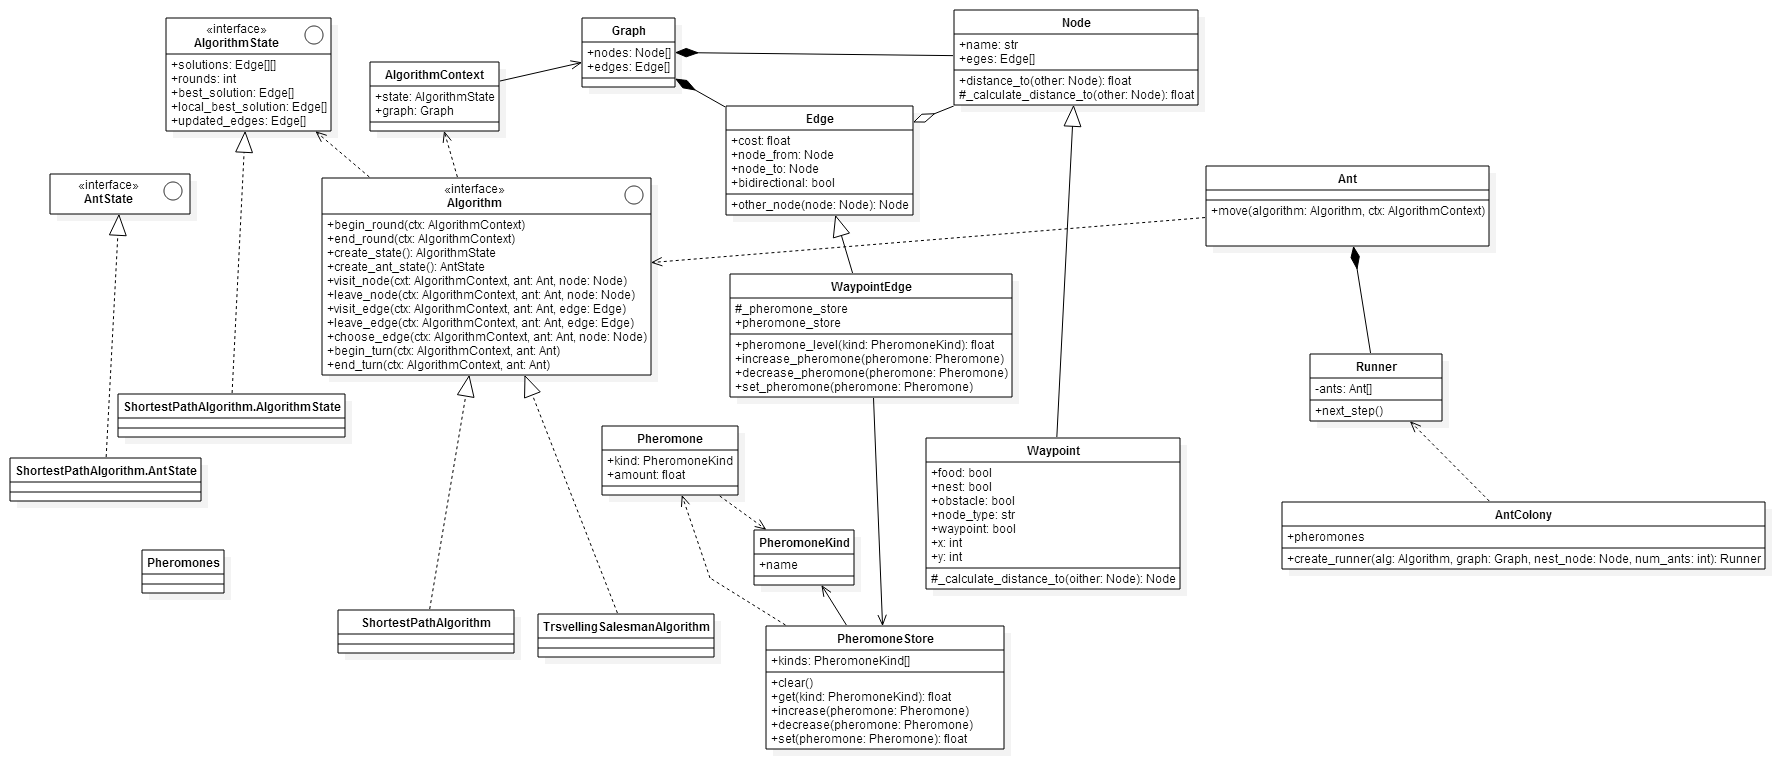
\includegraphics[width=0.85\textheight] {images/class_diagram.png}}
\caption{Klassendiagramm} 
\end{figure}

\pagebreak \subsubsection{Ergänzungen zum Klassendiagramm}

Dem Klassendiagramm kann entnommen werden, dass die einzelnen Klassen sehr lose
gekoppelt sind. So werden z.B. dem \texttt{Algorithm} Interface der
\texttt{AlgorithmContext}, die \texttt{Ant}, sowie der \texttt{Node} oder
\texttt{Edge} bei jedem Aufruf mitgegeben. Der \texttt{AlgorithmContext} enhält
zudem einen \texttt{state}, der zwar über die Factory-Methode
\texttt{Algorithm.create\_state()} erstellt wird, danach dem Algorithmus jedoch
bei jedem Aufruf übergeben wird. Damit kann für eine ganze Simulation eine
\texttt{Algorithm}-Instanz erstellt werden. Der \texttt{Algorithm} muss dadurch
auch bei der Neugenerierung des Graphen oder der Ameisen-Kolonie nicht mehr neu
instanziert werden.

\section{Vorgehen bei der Programmierung}

Wie unseren Release-Zusammenfassungen zu entnehmen ist, haben wir uns am Anfang
primär auf die Entwicklung einer lauffähigen Version mit graphischer Darstellung
konzentriert, in der sich Ameisen nach gewissen Regeln fortbewegen.

Danach haben wir uns auf die Implementation des korrekten Algorithmus fokussiert,
was sehr viel Zeit in Anspruch nahm und hauptsächlich ein Ausprobieren 
verschiedener Konfiguration beinhaltete.

Erst in der dritten Iteration wurde uns klar, dass verschiedene Teile des 
Algorithmus nicht akkurat wiedergegeben waren und das GUI zu wenig modular
programmiert, um weitere Funktionalität einzubauen. Dies führte zu einem gossen
Refactoring, welches schlussendlich gut verlaufen ist.

\section{Mockups}

Zwei verschiedene Varianten für das spätere Aussehen des Programms standen im
Vordergrund: eine mit der Einstellungsleiste im oberen Fensterbereich, eine
zweite mit den Einstellungen am rechten Seitenrand.

\begin{figure}[h] \centering 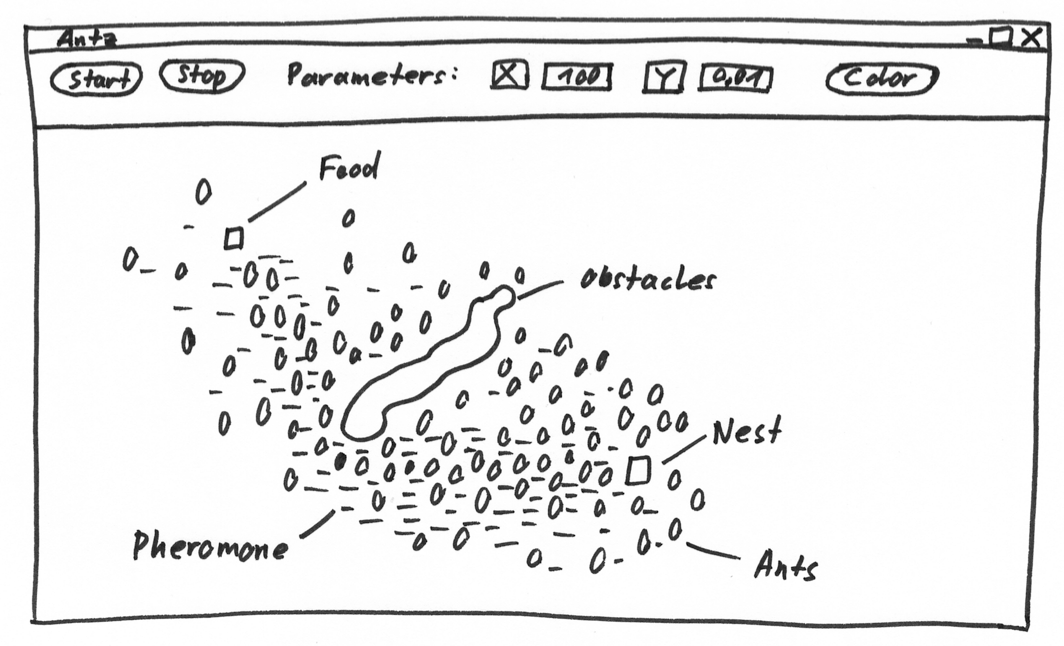
\includegraphics
[width=0.85\textwidth]{images/Antz_Mockup_1_sw.png} \caption{Mockup-Variante 1:
Einstellungen im oberen Fensterbereich} \end{figure}

\begin{figure}[h] \centering 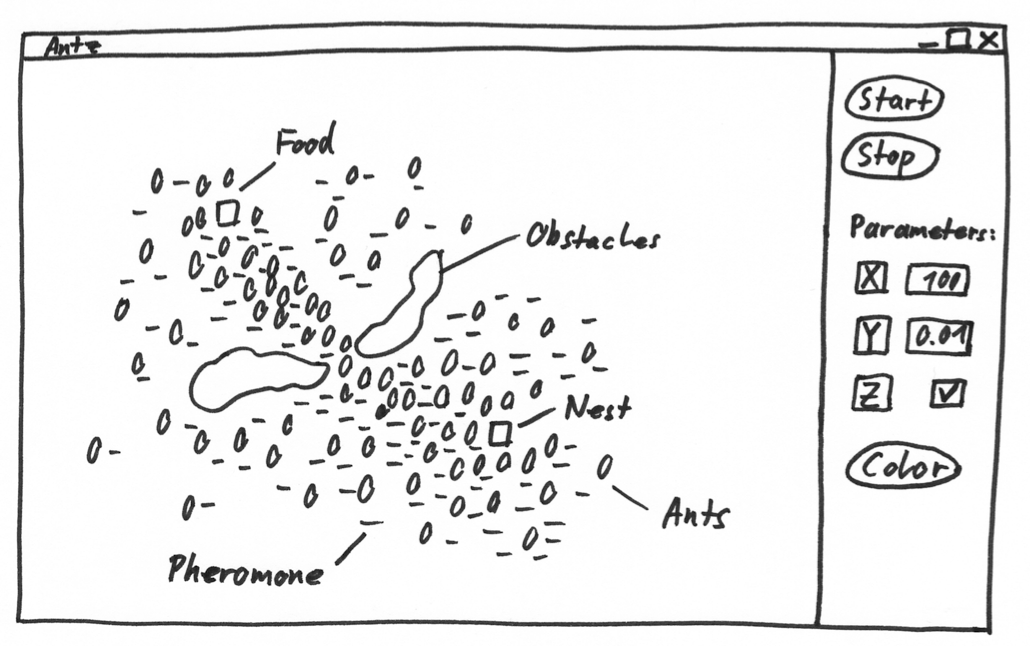
\includegraphics
[width=0.85\textwidth]{images/Antz_Mockup_2_sw.png} \caption{Mockup-Variante 2:
Einstellungen im rechten Fensterbereich} \end{figure}

\section{Bedienungsanleitung}

Der Programm kann durch Doppelklick auf \texttt{main.exe} im entpackten
\texttt{Antz.zip} Ordner gestartet werden (Abbildung \ref{fig:bedienung0}).

\begin{figure}[h] 
\centering 
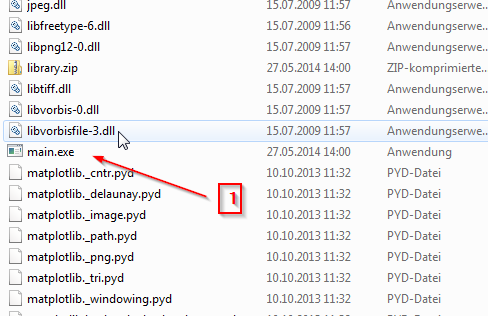
\includegraphics
[width=0.5\textwidth]{images/screenshots/bedienung_0.png} 
\caption{Starten durch Doppelklick auf main.exe} 
\label{fig:bedienung0}
\end{figure}

Das Programm startet und eine Oberfläche wie in Abbildung \ref{fig:bedienung1}
erscheint.

\begin{figure}[h] 
\centering 
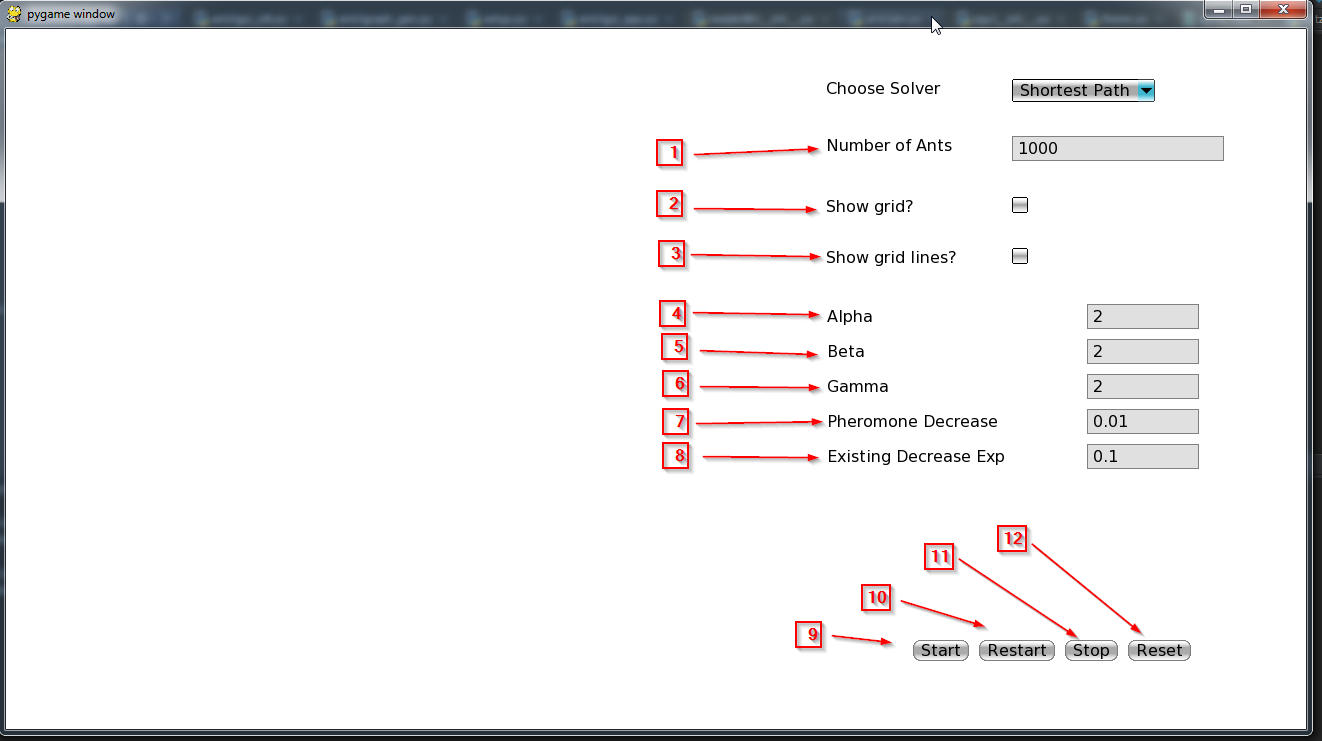
\includegraphics
[width=0.85\textwidth]{images/screenshots/bedienung_1.png} 
\caption{Oberfläche direkt nach dem Start des Programms} 
\label{fig:bedienung1}
\end{figure}

\begin{description}
\item[1] Die Anzahl Ameisen kann hier eingestellt werden. Es wird empfohlen, den
Wert unter 2000 zu halten, da das Programm ansonsten sehr langsam wird.
\item[2] Hier können Nodes ein- oder ausgeblendet werden. 
\item[3] Hier können Kanten ein- oder ausgeblendet werden.
\item[4] Ein hoher $\alpha$-Wert führt dazu, dass Pheromonmengen-Unterschiede
stärker ins Gewicht fallen.
\item[5] Ein hoher $\beta$-Wert führt dazu, dass die Ameisen sich verstärkt für
die Kante mit den geringsten Kosten entscheiden. Bei einem sehr hohen Wert (z.B.
20) begehen die Ameisen die längeren Diagonalen nicht mehr.
\item[6] Der $\gamma$-Wert beeinflusst die Pheromonmengen-Erhöhung auf einer
Kante. Ein hoher Wert vergrössert die Unterschiede zwischen langen und kürzeren
Pfaden.
\item[7] Steuert die Pheromon-Evaporation. Je höher der Wert, desto schneller
verschwinden die Pheromone auf den Kanten.
\item[8] Steuert, wie stark die existierende Menge an Pheromonen sich auf die
Verminderung der Erhöhung der Menge auswirkt. Ein höherer Wert führt zu
stärkerer Verminderung.
\item[9] Startet die Simulation.
\item[10] Startet die Simulation mit demselben Graph und eingezeichneten
Hindernissen neu.
\item[11] Pausiert die Simulation, kann mit Start weitergeführt werden.
\item[12] Reset generiert einen neuen Graph.
\end{description}

\noindent Sobald ein Graph mit Reset oder Start generiert wurde, können mit der linken
Maustaste Hindernisse gezeichnet werden. Mit der rechten Maustaste können sie
gelöscht werden.

\begin{figure}[H] 
\centering 
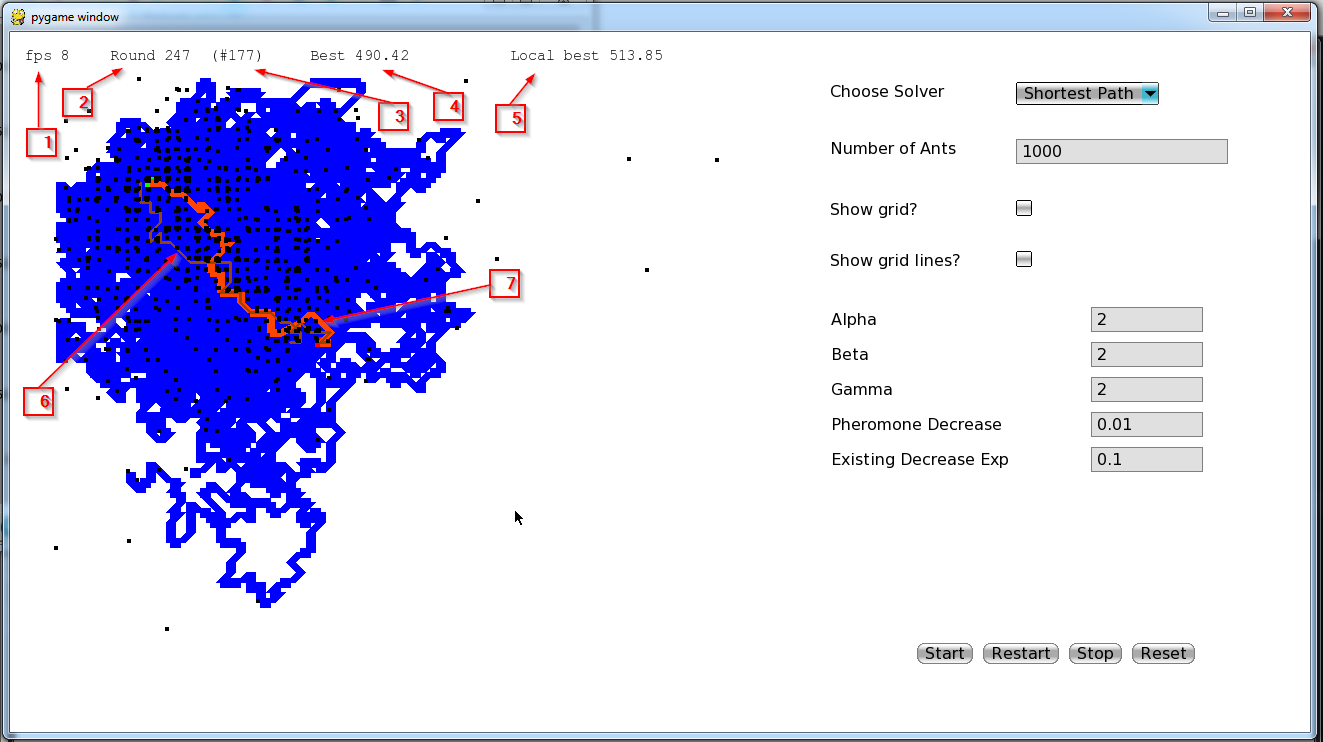
\includegraphics
[width=0.85\textwidth]{images/screenshots/bedienung_2.png} 
\caption{Oberfläche nach dem Start der Simulation}
\label{fig:bedienung2}
 \end{figure}

\noindent Abbildung \ref{fig:bedienung2} zeigt eine laufende Simulation.

\begin{description}
\item[1] Zeigt die Framerate an. 
\item[2] Zeigt an, wie viele Runden bereits gemacht wurden. Eine Runde
beinhaltet eine Bewegung aller Ameisen.
\item[3] Zeigt an, wie viele parallele Lösungen momentan existieren. Eine kleine
Zahl ($<100$) ist generell besser.
\item[4] Zeigt den insgesamt besten Pfad an, auch wenn sich momentan keine
Ameise auf diesem Pfad befindet.
\item[5] Zeigt den im Moment besten Pfad an, es befindet sich mindestens eine
Ameise auf diesem Pfad.
\item[6] Zeigt den im Moment besten Pfad graphisch an.
\item[7] Zeigt den insgesamt besten Pfad graphisch an.
\end{description}

\newpage

\vbox{
\subsection{Beispiele}

Es folgen zwei Beispiele, welche die Auswirkungen unterschiedlicher
$\alpha$-Werte demonstrieren sollen. Es wird der Stand nach 500 Schritten
aufgeführt.
}

\begin{table}[H]
\small\sffamily\renewcommand{\arraystretch}{1.5}
\begin{tabular}{ | r | r | r | r | } 
\hline $\alpha$ & Anzahl Lösungen & Beste Lösung & Lokal beste Lösung  \\ 
\hline 1 & 105 & 261.42 & 496.57 \\ 
\hline 2 & 193 & 290.71 & 290.71  \\ 
\hline 4 & 32 & 218.99 & 387.28  \\ 
\hline 10 & 3 & 278.99 & 315.56  \\ 
\hline \end{tabular}
\caption{Verschiedene $\alpha$-Werte} 
\end{table}

\noindent Bei der Suche nach der besten Lösung ist keine klare Tendenz zu erkennen. Alle 
Konfigurationen finden in etwa die gleiche Lösung. Nur konvergiert die Lösung bei 
hohen $\alpha$-Werten schnell zu sehr wenig unterschiedlichen Möglichkeiten. Dies 
führt dazu, dass der Algorithmus seine Flexibilität verliert. Alternative,
eventuell bessere Pfade können dadurch nicht mehr in Betracht gezogen werden. \\

\begin{figure}[H] 
\centering 
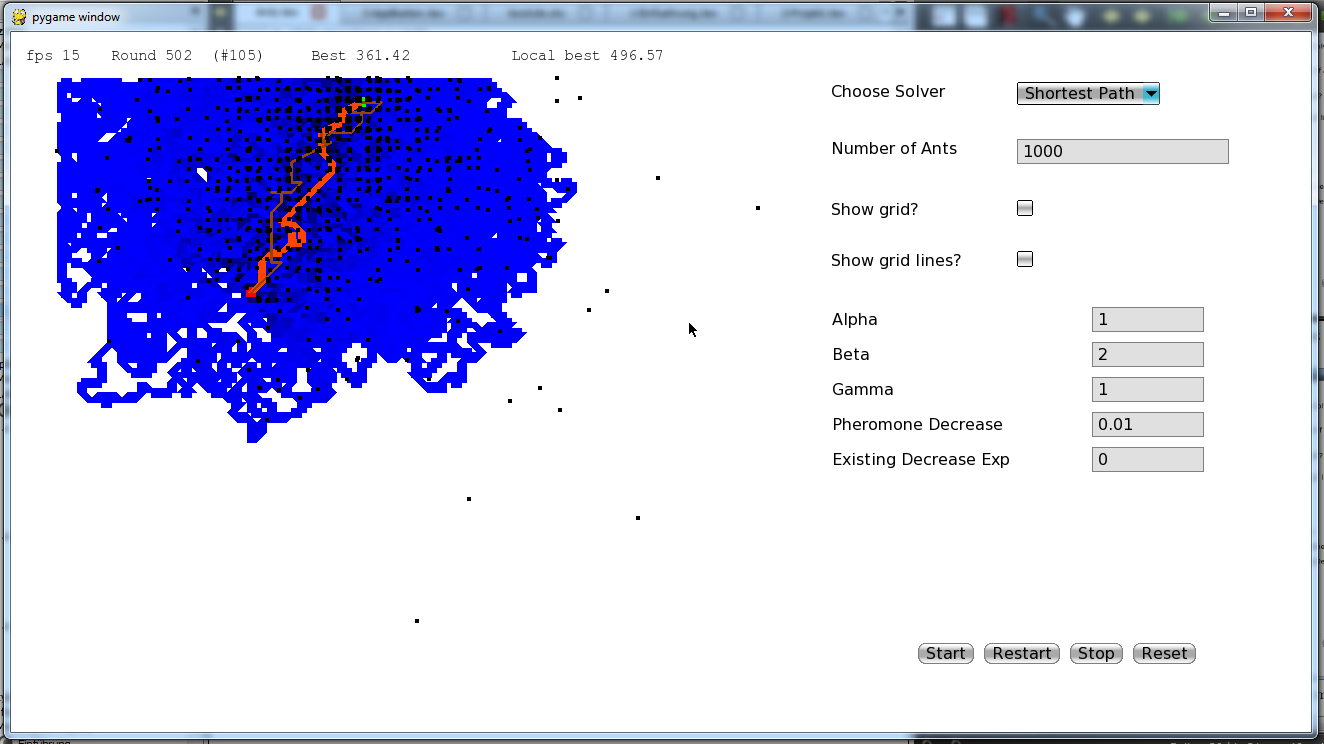
\includegraphics
[width=0.85\textwidth]{images/screenshots/eg_alpha_1.png} 
\caption{$Bespiel-Durchlauf mit \alpha = 1$} 
\label{fig:eg_alpha_1}
\end{figure}

\newpage

\begin{figure}[H] 
\centering 
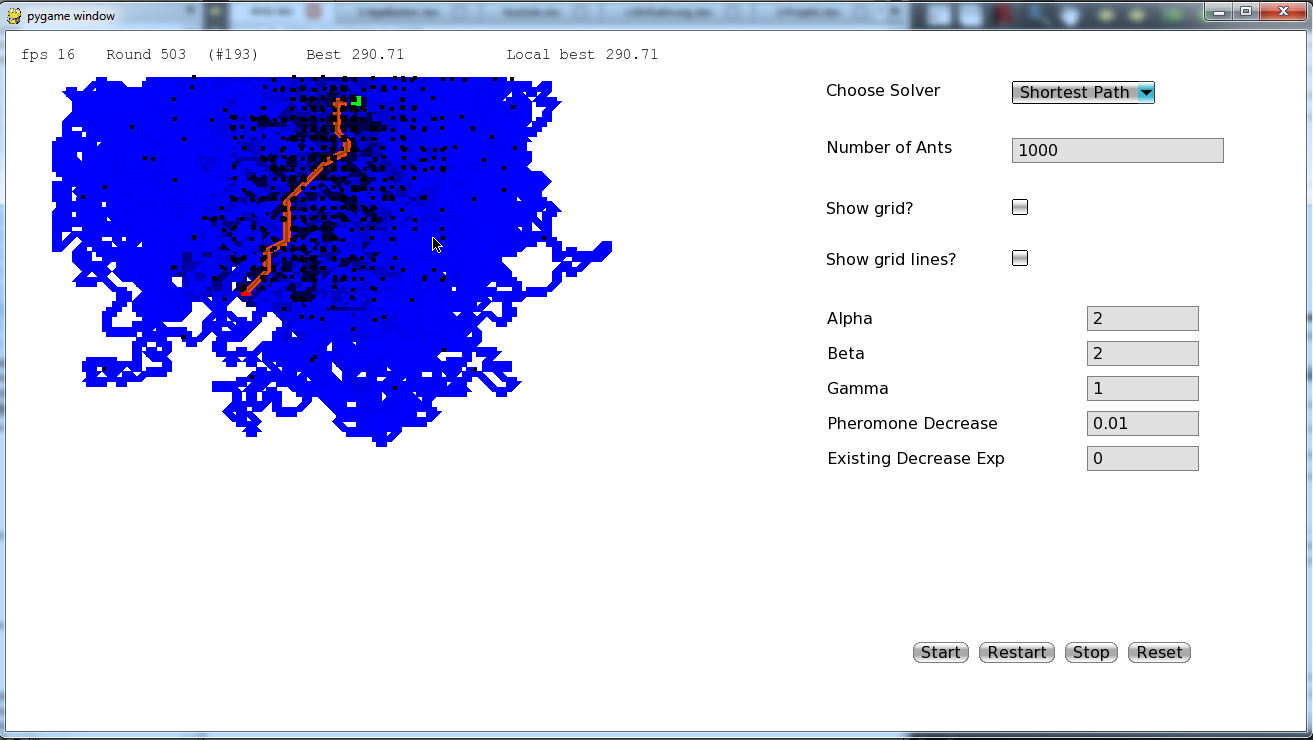
\includegraphics
[width=0.85\textwidth]{images/screenshots/eg_alpha_2.png} 
\caption{$Bespiel-Durchlauf mit \alpha = 2$} 
\label{fig:eg_alpha_2}
\end{figure}

\begin{figure}[H] 
\centering 
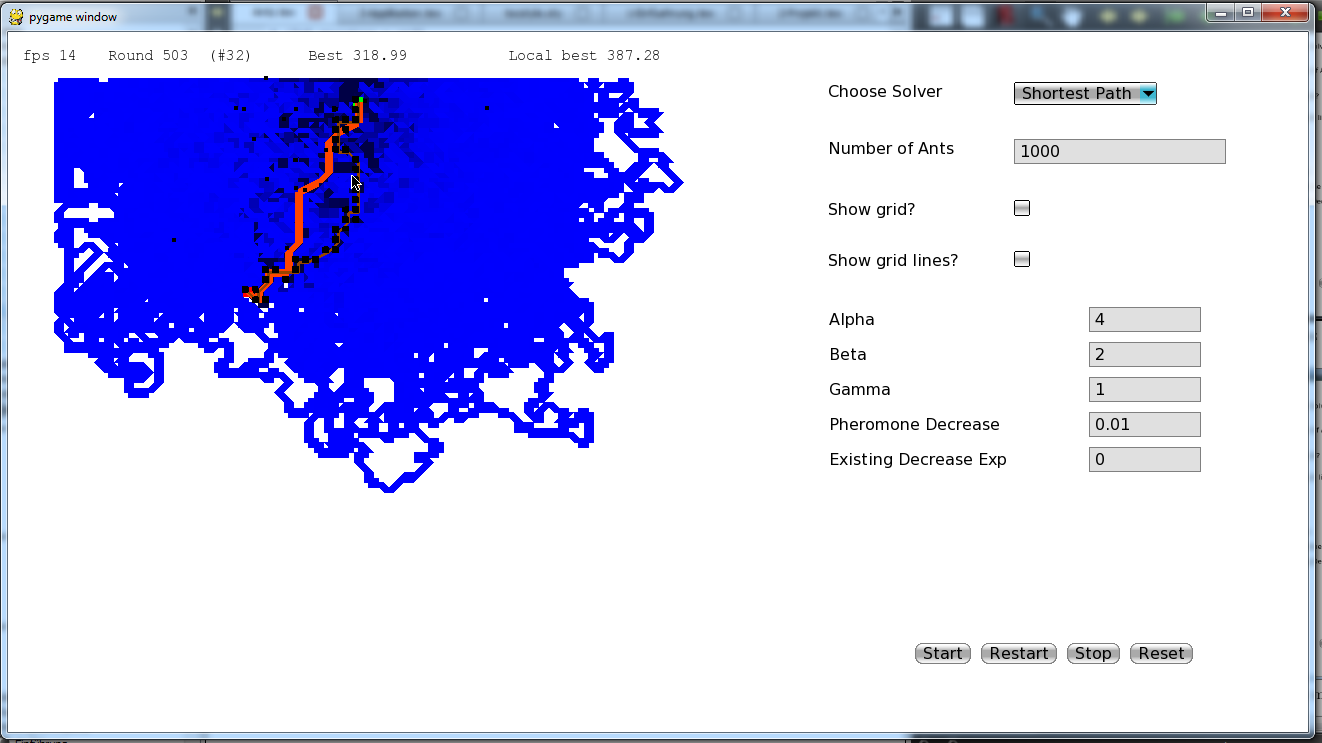
\includegraphics
[width=0.85\textwidth]{images/screenshots/eg_alpha_4.png} 
\caption{$Bespiel-Durchlauf mit \alpha = 4$} 
\label{fig:eg_alpha_4}
\end{figure}

\begin{figure}[H] 
\centering 
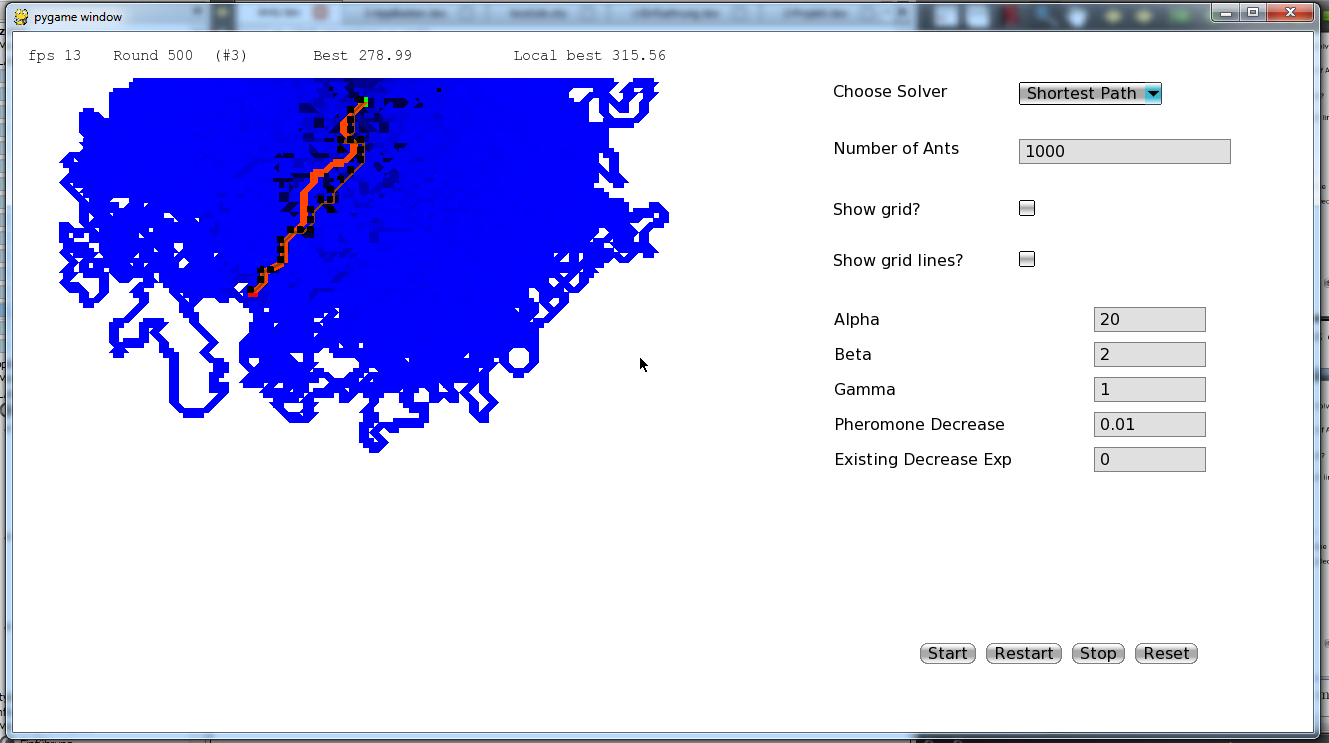
\includegraphics
[width=0.85\textwidth]{images/screenshots/eg_alpha_10.png} 
\caption{$Bespiel-Durchlauf mit \alpha = 10$} 
\label{fig:eg_alpha_10}
\end{figure}

\section{Vergleich mit Dijkstra und A*}

Im Rahmen dieser Projektarbeit wurde zwar kein Vergleich mit den Algorithmen von
Dijkstra oder A* aufgestellt, trotzdem soll hier kurz darauf eingegangen und
dafür die Resultate von \citet*{leo-perf} verwendet werden.

\citeauthor*{leo-perf} untersuchen die drei Algorithmen Dijkstra, A* und Ant auf
ihre Effizienz beim Finden eines kürzesten Pfades. Dabei gelangen sie zu
folgenden
Resultaten:

\begin{table}[h] 
\begin{tabular}{ | l | r | } 
\hline Dijkstra & $\sim\SI{140}{\milli\s}$ \\ 
\hline A* & $\sim\SI{110}{\milli\s}$ \\ 
\hline Ant & $\sim\SI{13900}{\milli\s}$  \\ 
\hline \end{tabular}
\caption{Vergleich zwischen Dijkstra, A* und Ant} 
\end{table}

\noindent Es lässt sich klar erkennen, dass der Ant-Algorithmus für die
Pfadfindung nicht besonders gut geeignet ist. Zu der höheren Ausführungszeit
kommt noch, dass Dijkstra und A* immer den optimalen Weg finden, der
Ant-Algorithmus jedoch nicht zwingend.

\citeauthor*{leo-perf} untersuchen auch die Eignung des Ant-Algorithmus für das
Travelling Salesman Problem und gelangen dabei zu ähnlichen Ergebnissen. Es ist
jedoch anzunehmen, dass sich der Ameisenalgorithmus bei sich dynamisch
verändernden Verhältnissen schneller anpassen kann. Dijkstra und A* müssen, wenn
z.B. ein Knoten wegfällt, alle Distanzen neu berechnen. Der Ameisenalgorithmus
dagegen nicht.

\newpage


\section{Schwierigkeiten}

Wir hatten bei der Programmierung einige Schwierigkeiten. Hier eine Auswahl:

\paragraph*{Algorithmus}

Wie im Kapitel \ref{sec:algorithm} besprochen, müssen verschiedene Werte auf das
Interval $[0,1]$ normiert werden. Dies haben wir erst sehr spät herausgefunden.
Somit waren die Ergebnisse, die wir erhielten, nicht konstant, wodurch wir durch
Debugging sehr viel Zeit verloren haben. Insbesondere haben wir relativ spät
(erst in der letzten Iteration) richtig verstanden, wie sich die Exponenten auf
die Wahrscheinlichkeiten auswirken.

\paragraph*{Performance}

Die Performance war lange sehr schlecht, wegen zu häufiger Iterationen über z.B.
die Kanten, um Pheromone zu evaporieren. Diese Probleme konnten jedoch bereits
in der zweiten Iteration behoben werden.

\paragraph*{Code-Stil und Refactorings}

Dadurch, dass wir das Game-Framework pyGame verwendet haben, ohne vorher damit
gearbeitet zu haben, sah unser GUI-Code schnell aus wie ein Auszug aus einem
Anfänger-Tutorial. Der Code war sehr unstrukturiert. In der letzten Iteration
mussten wir deswegen ein grösseres Refactoring vornehmen. Ansonsten wären die
Funktionalitäten wie Restart und Reset kaum möglich gewesen.

